\documentclass[acmsmall]{acmart}
\usepackage{subcaption}
\usepackage{float}

%%
%% \BibTeX command to typeset BibTeX logo in the docs
\AtBeginDocument{%
  \providecommand\BibTeX{{%
    \normalfont B\kern-0.5em{\scshape i\kern-0.25em b}\kern-0.8em\TeX}}}

%% Rights management information.  This information is sent to you
%% when you complete the rights form.  These commands have SAMPLE
%% values in them; it is your responsibility as an author to replace
%% the commands and values with those provided to you when you
%% complete the rights form.
\setcopyright{none}
\copyrightyear{2020}
\acmYear{2020}
\renewcommand\footnotetextcopyrightpermission[1]{}
\acmDOI{}
\pagestyle{plain}
\settopmatter{printacmref=false}


%%
%% Submission ID.
%% Use this when submitting an article to a sponsored event. You'll
%% receive a unique submission ID from the organizers
%% of the event, and this ID should be used as the parameter to this command.
%%\acmSubmissionID{123-A56-BU3}

%%
%% The majority of ACM publications use numbered citations and
%% references.  The command \citestyle{authoryear} switches to the
%% "author year" style.
%%
%% If you are preparing content for an event
%% sponsored by ACM SIGGRAPH, you must use the "author year" style of
%% citations and references.
%% Uncommenting
%% the next command will enable that style.
%%\citestyle{acmauthoryear}

%%
%% end of the preamble, start of the body of the document source.
\begin{document}

%%
%% The "title" command has an optional parameter,
%% allowing the author to define a "short title" to be used in page headers.
\title{Author Attribution: DerStandard Forum Writing Style}

%%
%% The "author" command and its associated commands are used to define
%% the authors and their affiliations.
%% Of note is the shared affiliation of the first two authors, and the
%% "authornote" and "authornotemark" commands
%% used to denote shared contribution to the research.
\author{Patrick Deutschmann}
\email{patrick.deutschmann@tugraz.at}

\author{Lukas Timpl}
\email{lukas.timpl@tugraz.at}


%%
%% The abstract is a short summary of the work to be presented in the
%% article.
\begin{abstract}
  %TODO write abstract
\end{abstract}

%%
%% The code below is generated by the tool at http://dl.acm.org/ccs.cfm.
%% Please copy and paste the code instead of the example below.
%%
\begin{CCSXML}
<ccs2012>
   <concept>
       <concept_id>10010147.10010178.10010179</concept_id>
       <concept_desc>Computing methodologies~Natural language processing</concept_desc>
       <concept_significance>500</concept_significance>
       </concept>
 </ccs2012>
\end{CCSXML}

\ccsdesc[500]{Computing methodologies~Natural language processing}
%%
%% Keywords. The author(s) should pick words that accurately describe
%% the work being presented. Separate the keywords with commas.
\keywords{natural language processing, neural networks, author attribution, RNN}


%%
%% This command processes the author and affiliation and title
%% information and builds the first part of the formatted document.
\maketitle

\section{Problem Setting}

The aim of this project is to identify the authors of posts to a newspaper forum. This should be achieved through the incorporation of multiple factors, such as writing style and content, but also meta information such as the post date and the article to which the post was written. In that, the setting differentiates itself from the classical authorship attribution setting, where no meta information is used. 

The dataset we used for this project was the One Million Posts Corpus, provided by \cite{MillionPosts}. It contains user comments in German language posted for the Austrian newspaper DerStandard\footnote{\url{https://www.derstandard.at}}.

The concrete problem was formulated such that given a new post and its meta information, the most likely author of all forum users should be predicted. For that we only considered the most active users with at least 500 posts. There were in total 212 user for which this was the case in our data set.

\section{Related Work}

Authorship attribution is an actively researched field with many different special areas to focus on. While more traditional, manual methods such as described in \cite{criminalForensics} largely focus on linguistic expert analysis, more modern approaches make use of computers to solve the problem.

Much research effort, such as in \cite{rexha2015towards,sanderson2006short}, is focused on author attribution of far longer texts than the short ones given in our comments section. However, in \cite{smith2009authorship,macleod2012whose} there is some analysis of short texts with methods that are also applicable to our use case. 

This project differentiates itself from the aforementioned papers as it not only considers the writing style to determine the author, but also incorporates the meaning of the written text and some additional meta information, rendering it a significantly easier task.

\section{Setup}
%TODO @Patrick

% This project explores different methods of identifying the authors of these posts...
% - focused on MLP because it makes sense for this task (left other architectures for future work)


\section{Features}
To best utilize our dataset we made use of various different features which are described in this section. 

\subsection{Post Metadata}
The dataset contains a number of values we consider as meta-data, data that is not directly related to the actual text of the post and can be computed without considering the actual content of the post. 

\subsubsection{Date Statistics}
For this feature we analysed at which time of the day and on which day of the week users write their posts. 
The notion behind this was, that individual users will tend to at similar times.
A histogram of this data is depicted in Figure~\ref{fig:date_stats}.

\begin{figure}[H]
\centering
\begin{subfigure}{.5\textwidth}
\centering
  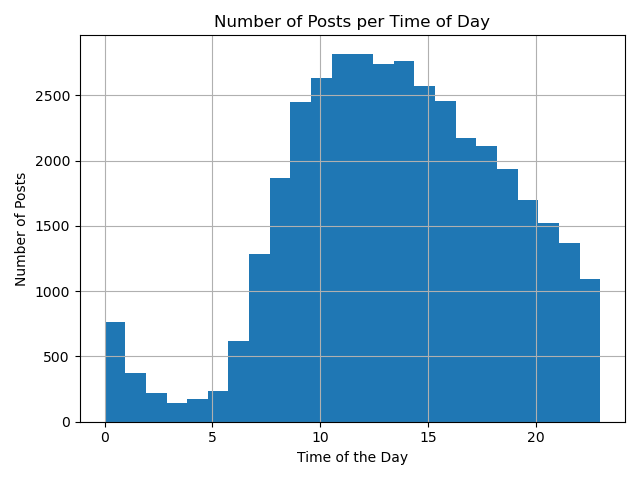
\includegraphics[width=.9\linewidth]{assets/Number_of_posts_per_time_of_day.png}
 \end{subfigure}%
\begin{subfigure}{.5\textwidth}
\centering
  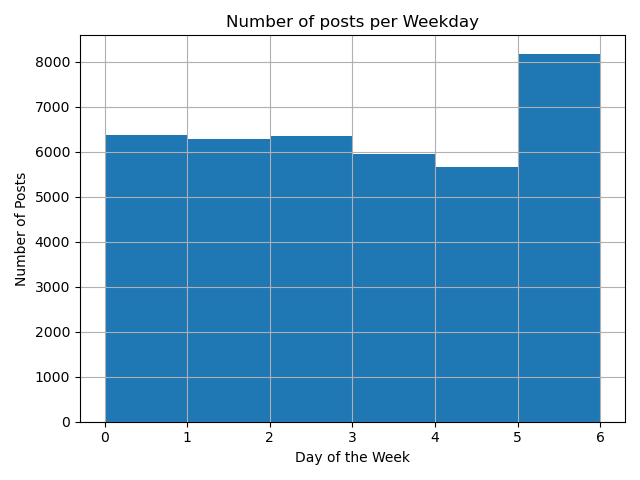
\includegraphics[width=.9\linewidth]{assets/Number_of_posts_per_day_of_week.png}
 \end{subfigure}
 \caption{Date Statistics}
\label{fig:date_stats}
\end{figure}

\subsubsection{Post Ratings and Parent Posts}
For further information about a post without the actual content we looked at the post ratings and whether the post was a comment to another users post. The aim with this feature was to identify users that post more controversial content as well as users that only ever post comments (have a parent post) and users that never answer to other users (no parent post). Again we depict a histogram over this data (Figure~\ref{fig:post_stats}). This figure clearly shows, that most posts get no votes at all, while there are a few posts which get a very large number of votes. 

\begin{figure}[H]
\centering
\begin{subfigure}{.5\textwidth}
\centering
  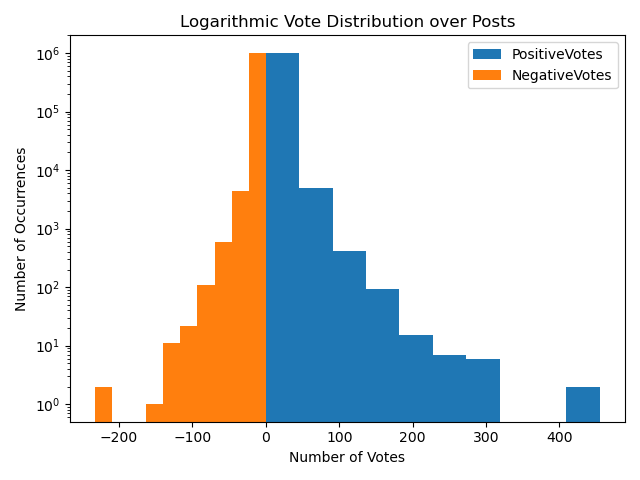
\includegraphics[width=.9\linewidth]{assets/Logarithmic_Vote_Distribution_over_Posts.png}
 \end{subfigure}%
\begin{subfigure}{.5\textwidth}
\centering
  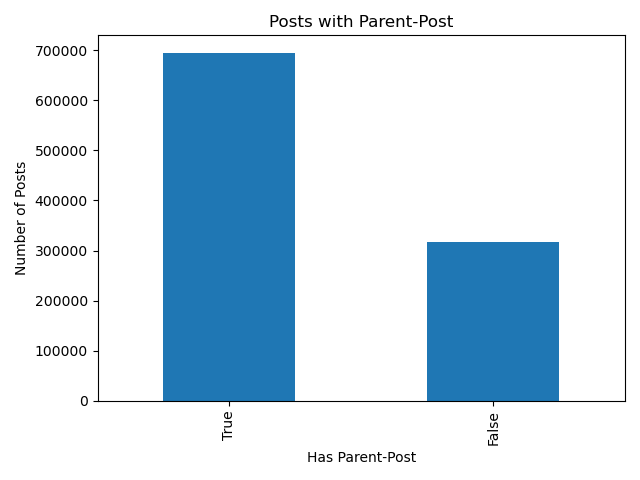
\includegraphics[width=.9\linewidth]{assets/Posts_with_parent_post.png}
 \end{subfigure}
 \caption{Post Statistics}
\label{fig:post_stats}
\end{figure}

\subsubsection{Article Categories}
Articles in the dataset also contain a path which we used as a categorical feature with the idea, that individual users will be more interested in particular topics and therefore are more likely to write post under those articles. A histogram of the number of articles in each category of the most common main category "Newsroom" is depicted in Figure~\ref{fig:article_categories}.

\begin{figure}[H]
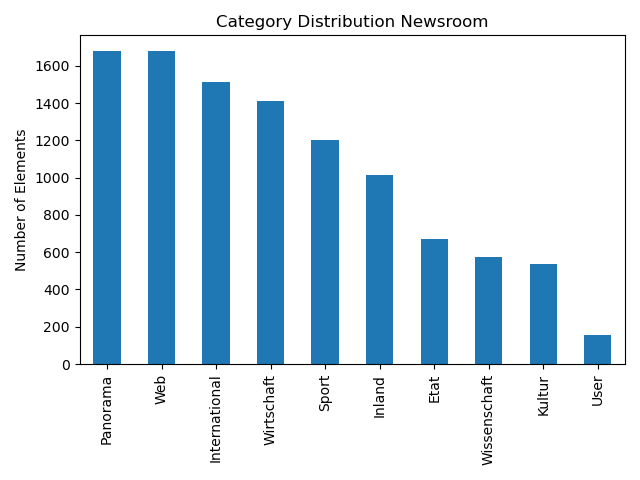
\includegraphics[width=.5\linewidth]{assets/Category_Distribution_Newsroom.png}
\caption{Article Category Distribution}
\label{fig:article_categories}
\end{figure}


\subsubsection{Article Named Entities}
To get a more detailed view of the interests of users additionally to the Article Categories, we also analysed Named Entities in the articles under which the posts where written. Similarly to the Article Categories, the notion behind this was, that individual users will be more interested in certain entities and hence are more likely to write a post under Articles containing these Entities. \\
For this we utilized the library Flair (\url{https://github.com/flairNLP/flair}) a library that offers state-of-the-art Named Entity Recognition for German language. Histograms for the most frequently recognized entities are depicted in Figure~\ref{fig:named_entities}. We only used entities that occurred at least 20 times. We count the occurrences of each entity and encode each article as a vector containing all entity counts. 

\begin{figure*}[h!]
        \centering
        \begin{subfigure}[b]{0.475\textwidth}
            \centering
            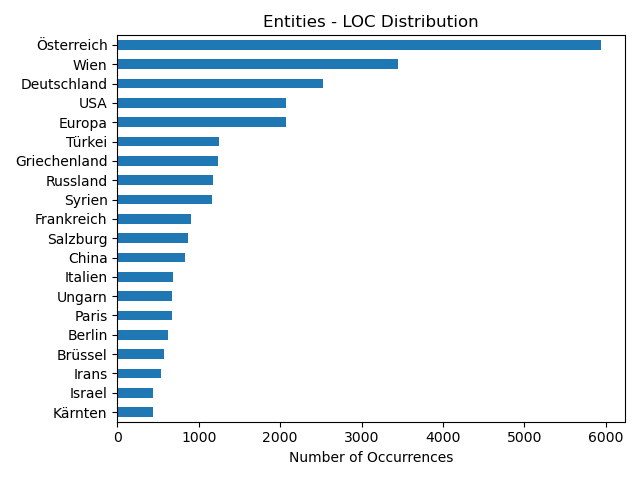
\includegraphics[width=\textwidth]{assets/Entities_LOC_Distribution.png}
        \end{subfigure}
        \begin{subfigure}[b]{0.475\textwidth}  
            \centering 
            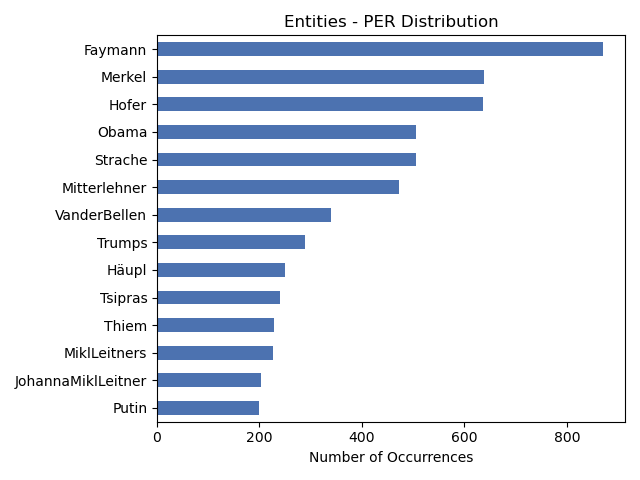
\includegraphics[width=\textwidth]{assets/Entities_PER_Distribution.png}
        \end{subfigure}
        \begin{subfigure}[b]{0.475\textwidth}   
            \centering 
            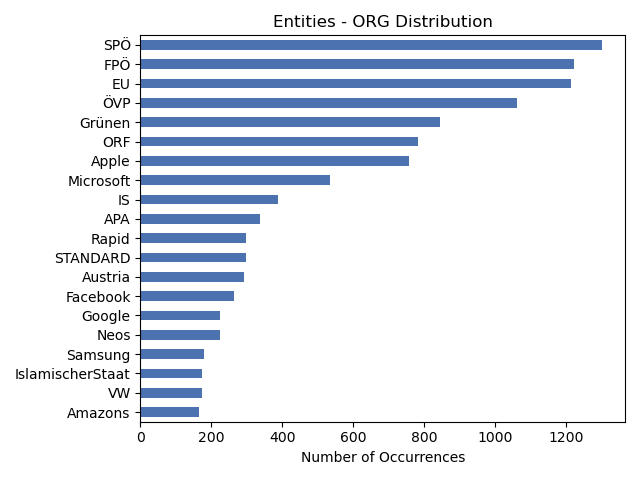
\includegraphics[width=\textwidth]{assets/Entities_ORG_Distribution.png}
        \end{subfigure}
        \begin{subfigure}[b]{0.475\textwidth}   
            \centering 
            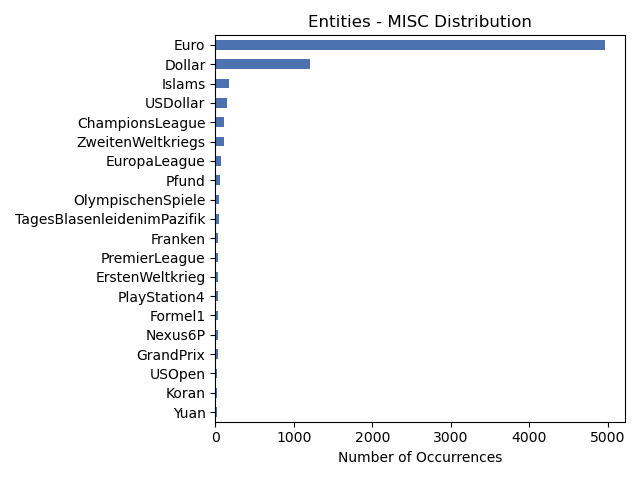
\includegraphics[width=\textwidth]{assets/Entities_MISC_Distribution.png}
        \end{subfigure}
         \caption{Top Entities in Articles for locations (LOC), persons (PER), organizations (ORG) and other Entities (MISC).}
         \label{fig:named_entities}
\end{figure*}


\subsection{Stylometric}
Next, we looked at the content of the posts and computed various stylometric features. These features are based on the writing style of the user. The list and description of these features can be found in Table~\ref{tab:stylometric}. We computed all of those features twice. Once for the headline of the post and once for the actual text. The notion behind this is, that we noticed, that the way in which the headline was used differed significantly between users. While some users choose to leave the field empty, some showed a clear tendency towards upper-case characters, and some wrote the headline as the start for the main text and concluded it with "...". 

\begin{table}[H]
\begin{tabular}{ll}
Feature Name & Description \\ \hline
Alpha-chars-ratio & The fraction of total characters in the paragraph which are letters \\
Digit-chars-ratio & The fraction of total characters in the paragraph which are digits \\
Upper-chars-ratio & The fraction of total characters in the paragraph which are upper-case \\
White-chars-ratio & The fraction of total characters in the paragraph which are whitespaces \\
Emoticon-chars-ratio & The number of Emoticons (e.g. ":)", ":D", ...) per total characters \\
Average-word-length & Average length of words in characters \\
Average-sentencechar-length & Average length of sentences in characters \\
Average-sentenceword-length & Average length of sentences in words \\
Total length & The length of the text \\
\end{tabular}
\caption{Used Stylometric Features}
\label{tab:stylometric}
\end{table}

\subsection{Post Embeddings}
As a final feature, we computed word embeddings for the post texts. The goal of this feature is to get information on the actual content the users write about as well as potentially additional information on their writing style. \\
To compute the vectors, we utilized the Word2Vec model of the library Gensim (\url{https://radimrehurek.com/gensim/}). 
We used embedding vectors of size 50 only computed the embedding for words which at least occurred ten times and trained the model over 500 iterations. 
When embedding the posts, we only embedded at most 100 words for each post to restrict the size of the feature.  

\section{Evaluation}
In this section we describe our results. For the final training of the network we split into a test and training set (80\%/20\%). Additionally we used a validation data set for early stopping (20\%) of the training test. 

\subsection{Baseline}
%TODO find more baseline data
As one base line we use random guessing. In our dataset we have 192 Users, hence a random guess yields an accuracy of $1/192 = 0.0052$. 

\subsection{Results}
In this section we list the achieved results for various feature configuration.
We first trained models for each individual feature the corresponding results are listed in Table~\ref{tab:result_features}. 
Next we trained different configurations containing various combination of features, the results are depicted in Table~\ref{tab:result_configurations}.

\subsubsection{Individual Features}
To get an idea of the usefulness of individual features we trained the network for each individual feature. 

For all features below we trained a simple network using an input layer, one or two hidden layers and one output layer. 
The results for each feature and the corresponding parameters are listed in Table~\ref{tab:result_features}.

\begin{table}[H]
\begin{tabular}{lllllll}
Feature & Val. Acc. & Test Acc. & Layers & Dropout & Learning Rate & Epochs\\ \hline
Date Stats & 0.041 & 0.047 & (256) & - & 0.2 & 20 \\
Post Ratings & 0.042 & 0.044 & (512) & - & 0.2 & 4 \\
Parent Post & 0.041 & 0.039 & (256) & - & 0.2 & 7 \\
Article Categories & 0.090 & 0.087 & (190) & - & 0.1 & 8 \\
Article Entities & 0.26 & 0.26 &  (700)  & - & 0.2 & 6 \\
Stylometric & 0.21 & 0.21 & (150),(512) & - & 0.1 & 18 
\end{tabular}
\caption{Results for individual features}
\label{tab:result_features}
\end{table}


\subsubsection{Metadata Features}
The notion behind this model was to use all available features that are not related to the content of the post. \\
Therefore the following features are used:
\begin{itemize}
\item Date Statistics
\item Post Ratings
\item Parent Posts
\item Article Categories
\item Article Named Entities
\end{itemize}

\subsubsection{Dense Features}
This model contains all features except for the embeddings. Since we added recurrent layers for the post embeddings this is the configuration with all features such that the model is still a feed forward network. 


\subsubsection{Post Content Features}
Since this model utilized the Post Embeddings we added recurrent layers and a concatenation layer to merge them with the remaining features which are only used in a feed forward manner. 
The model is depicted in Figure~\ref{fig:post_content_model}.
This model contains all features which are directly related to the content of the post.
Therefore the following features are used:
\begin{itemize}
\item Post Embeddings
\item Stylometrics
\end{itemize}


\subsubsection{All Features}
For this model we combined all available features. We used a recurrent network for the post embeddings and combined it with a feed forward network of the other features. The model is depicted in Figure~\ref{fig:complete_model}.


\begin{table}[H]
\begin{tabular}{lllllll}
Configuration & Val. Acc. & Test Acc. & Layers & Dropout & Learning Rate & Epochs\\ \hline
Metadata Features & 0.28 & 0.27 & (512) &  - & 0.2 & 18 \\
Dense Features & 0.36 & 0.35 & (90),(512) & - & 0.2 & 12 \\
Post Content Features & 0.32 & 0.31 & Fig.~\ref{fig:post_content_model} & 0.3 & 0.2 & 8 \\
All Features & 0.45 & 0.44 & Fig.~\ref{fig:complete_model} & 0.3 & 0.2 & 11 \\
\end{tabular}
\caption{Results for Configurations}
\label{tab:result_configurations}
\end{table}

\begin{figure}[H]
\centering
\begin{subfigure}{.5\textwidth}
\centering
  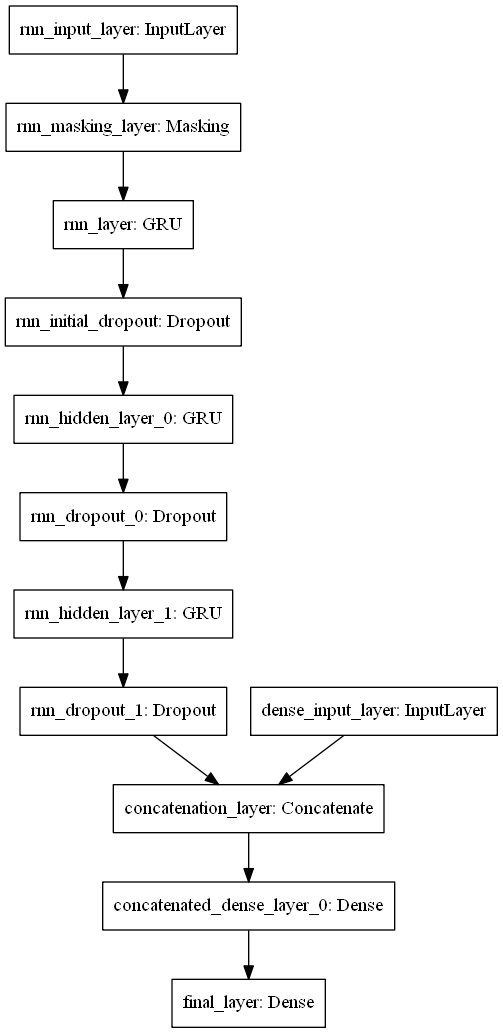
\includegraphics[width=.9\linewidth]{assets/AuthorAttributionModel_post_content_features.png}
  \caption{Model for Post Content Features}
  \label{fig:post_content_model}
 \end{subfigure}%
\begin{subfigure}{.5\textwidth}
\centering
  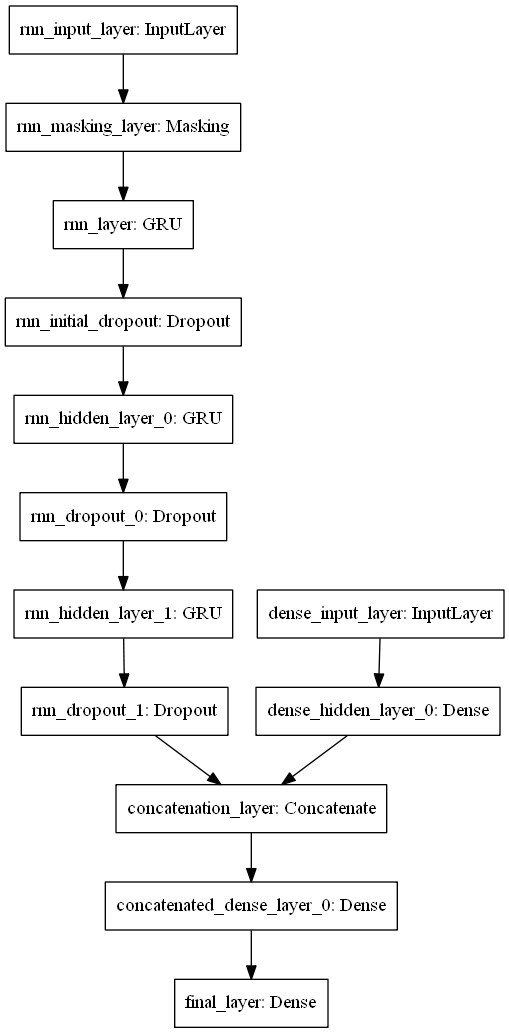
\includegraphics[width=.9\linewidth]{assets/AuthorAttributionModel_all_features.png}
  \caption{Complete Model for all features}
    \label{fig:complete_model}
 \end{subfigure}
 \caption{RNN Models}
\label{fig:rnn_models}
\end{figure}


\section{Discussion}
%TODO

\section{Conclusion}
%TODO

% TODO write about future work:
% - try architectures other than Neural Network (MLP)
% - comparison with other methods

\pagebreak

%%
%% The next two lines define the bibliography style to be used, and
%% the bibliography file.
\bibliographystyle{ACM-Reference-Format}
\bibliography{references}


\end{document}
\endinput

